\documentclass[tikz,border=6pt]{standalone}

\usepackage{tikz}
\usetikzlibrary{math}

\begin{document}

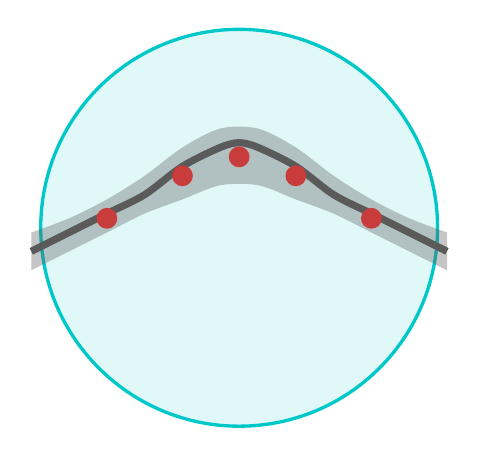
\begin{tikzpicture}[scale=1.2]

% === Colors ===
\definecolor{cyanfill}{RGB}{0,200,200}
\definecolor{grayline}{RGB}{90,90,90}
\definecolor{reddots}{RGB}{200,60,60}

% === Outer circle (very light cyan fill) ===
\fill[cyanfill, opacity=0.12] (0,0) circle (2.1);
\draw[cyanfill, line width=1.2pt] (0,0) circle (2.1);

% === Confidence interval band (gray, opaque) ===
\fill[grayline, opacity=0.35]
  plot[smooth] coordinates {
    (-2.2,-0.05) (-1.8,0.10) (-1.4,0.30) (-1.0,0.55)
    (-0.6,0.85) (-0.2,1.05) (0.2,1.05) (0.6,0.85)
    (1.0,0.55) (1.4,0.30) (1.8,0.10) (2.2,-0.05)
  }
  --
  plot[smooth] coordinates {
    (2.2,-0.45) (1.8,-0.25) (1.4,-0.05) (1.0,0.15)
    (0.6,0.30) (0.2,0.45) (-0.2,0.45) (-0.6,0.30)
    (-1.0,0.15) (-1.4,-0.05) (-1.8,-0.25) (-2.2,-0.45)
  }
  -- cycle;

% === Gaussian distribution line ===
\draw[grayline, line width=2.6pt, smooth]
  plot coordinates {
    (-2.2,-0.25) (-1.8,-0.05) (-1.4,0.15) (-1.0,0.35)
    (-0.6,0.65) (-0.2,0.85) (0.0,0.90) (0.2,0.85)
    (0.6,0.65) (1.0,0.35) (1.4,0.15) (1.8,-0.05)
    (2.2,-0.25)
  };

% === Ensemble points (red, inside CI) ===
\foreach \x/\y in {
  -1.4/0.10,
  -0.6/0.55,
   0.0/0.75,
   0.6/0.55,
   1.4/0.10
}{
  \fill[reddots] (\x,\y) circle (0.11);
}

\end{tikzpicture}


\end{document}
